\chapter{Continuous Reactors and Industrial Processes}\label{ch:b2:continuous-reactors}

In the laboratory a reaction is run in a flask: the reagents go in, the
mixture is stirred for an hour, the reaction is stopped and the product
isolated. A plant that makes the same product by the thousand tonnes works
differently. Its reactor never empties: reactants flow in at one end,
products flow out at the other, day and night, and the composition inside
does not change with time. Two questions then replace ``how long?'': how
large must the reactor be for a given \omterm{def:b2:continuous-reactors:conversion}{conversion}, and how is the heat of
the reaction taken away before it heats the reactor out of control? This
chapter writes the balances of matter and energy for the two ideal
\omterm{def:b2:continuous-reactors:reactors}{continuous reactors}, the stirred tank and the tube, compares them, and
shows how a reactor can have several possible states, one of them a
runaway.

\begin{recall}
The Year 1 volume: rate of reaction, rate laws and orders, integrated laws
of a closed reactor (now called a \omterm{def:b2:continuous-reactors:reactors}{batch reactor}), half-life, the Arrhenius
law $k = A\,\mathrm e^{-E_a/RT}$, consecutive reactions.
\Cref{ch:b2:reaction-enthalpy}: heat released at constant pressure;
\cref{ch:b2:equilibrium-shifts}: \omterm{def:b2:equilibrium-shifts:single-pass}{single-pass conversion}, \omterm{def:b2:equilibrium-shifts:single-pass}{recycle}. From
physics: the balance of an open system in steady flow (what enters minus
what leaves equals what accumulates).
\end{recall}

\begin{omfigure}
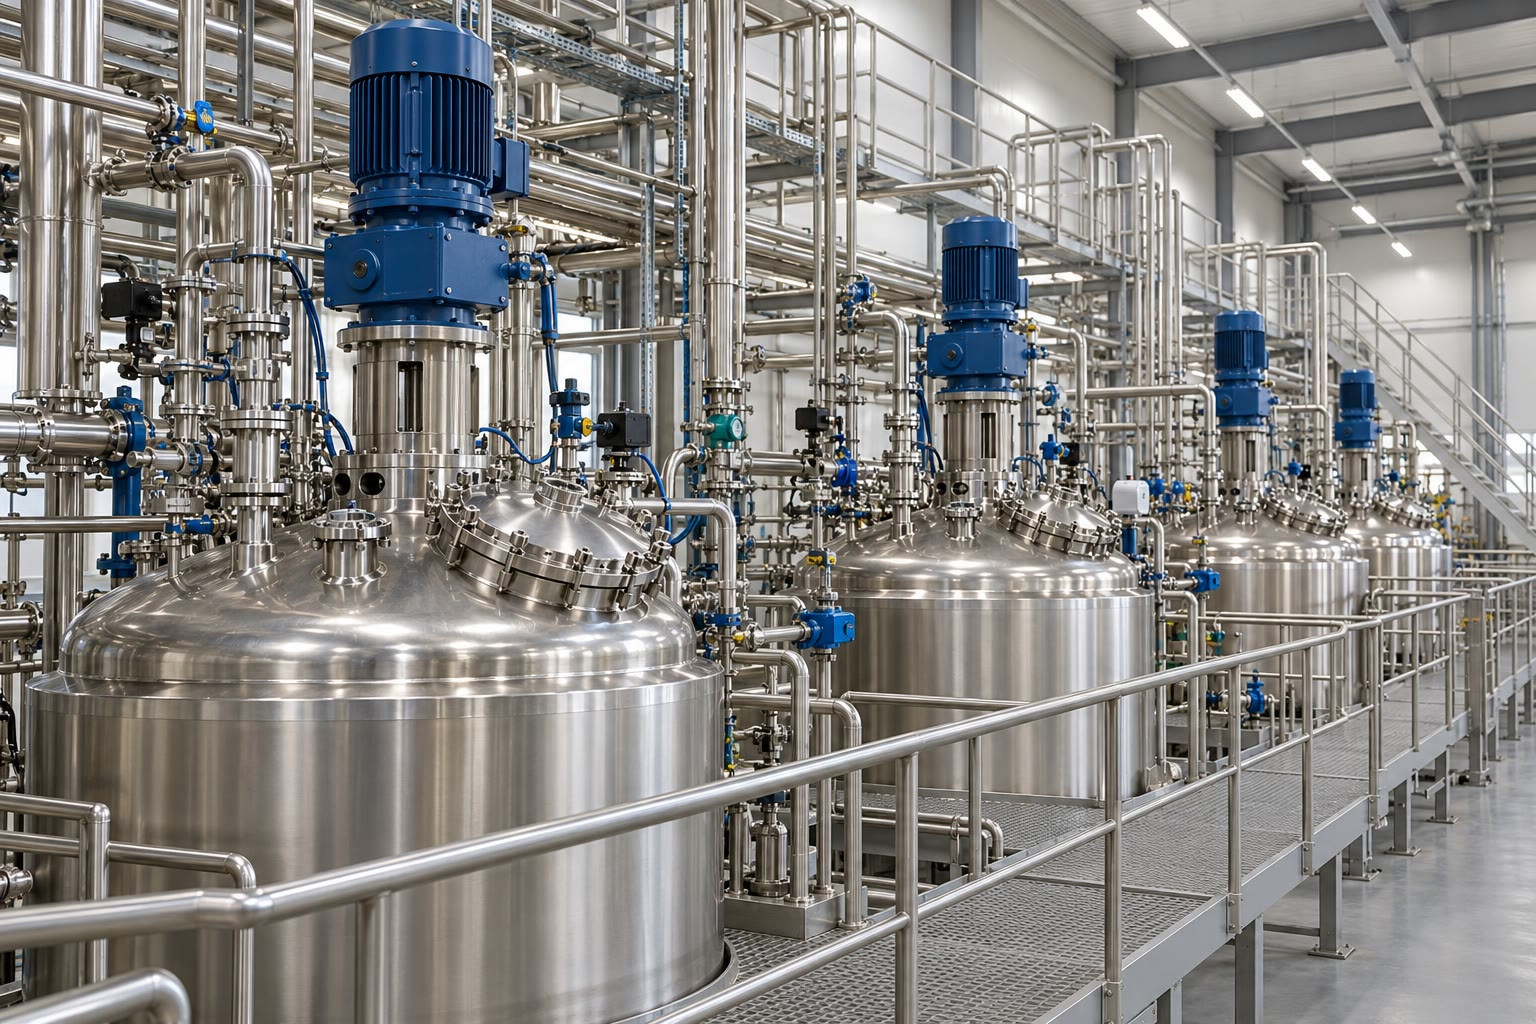
\includegraphics[width=0.6\linewidth]{images/book3/ai/b2-05-stirred-tanks.jpg}

{\small Stirred-tank reactors in a chemical plant: each vessel carries its
motor and gearbox, the stirrer shaft going down into the reaction mixture;
the pipes bring the feeds and take the product and the cooling water.}
\end{omfigure}

\section{From batch to continuous}

\begin{definition}[Reactor types]\label{def:b2:continuous-reactors:reactors}
A \emph{batch reactor}\index{batch reactor} is a closed vessel in which the
reaction takes place without inflow or outflow of matter. A
\emph{continuous reactor}\index{continuous reactor} is crossed by a steady
flow of matter. Two ideal continuous reactors serve as models:
\begin{itemize}
  \item the \emph{continuous stirred-tank reactor}\index{continuous
        stirred-tank reactor} (CSTR), so well stirred that its contents are
        uniform, and therefore identical to the stream that leaves it;
  \item the \emph{plug-flow reactor}\index{plug-flow reactor} (PFR), a tube
        crossed by the fluid without mixing along the flow, each slice of
        fluid advancing like a piston while it reacts.
\end{itemize}
\end{definition}

A \omterm{def:b2:continuous-reactors:reactors}{continuous reactor} is said to work in \emph{steady operation} when
nothing inside it changes with time: the flows, the temperatures and the
compositions at each point are constant. We consider a single reaction
$\mathrm A \to$ products, a liquid feed of constant density (so the
volumetric flow rate $Q_v$ is the same at the inlet and outlet), with
concentration $c_{A,0}$ at the inlet.

\begin{definition}[Residence time]\label{def:b2:continuous-reactors:residence-time}
The \emph{residence time}\index{residence time} of a \omterm{def:b2:continuous-reactors:reactors}{continuous reactor} of
volume $V$ fed at the volumetric flow rate $Q_v$ is $\tau = V/Q_v$: the mean
time a volume of fluid spends inside it.
\end{definition}

\begin{definition}[Conversion]\label{def:b2:continuous-reactors:conversion}
The \emph{conversion}\index{conversion} of reactant A is $X = (F_{A,0} -
F_A)/F_{A,0}$, where $F_{A,0}$ and $F_A$ are the molar flow rates of A
entering and leaving the reactor; for a \omterm{def:b2:continuous-reactors:reactors}{batch reactor}, $X = (n_{A,0} -
n_A)/n_{A,0}$. At constant density, $X = 1 - c_A/c_{A,0}$.
\end{definition}

\omterm{def:b2:continuous-reactors:conversion}{Conversion} refers to one reactant, and to a reactor or a pass; the final
fractional extent of the Year 1 volume refers to a reaction and to its
limiting reactant. For a single reaction whose limiting reactant is A, the
two coincide.

\begin{proposition}[Batch reactor]\label{prop:b2:continuous-reactors:batch}
In a \omterm{def:b2:continuous-reactors:reactors}{batch reactor} of constant volume, a first-order reaction reaches the
\omterm{def:b2:continuous-reactors:conversion}{conversion} $X = 1 - \mathrm e^{-kt}$ after the time $t$, and a second-order
reaction with equal initial concentrations $c_0$ the \omterm{def:b2:continuous-reactors:conversion}{conversion} $X =
kc_0t/(1 + kc_0t)$.
\end{proposition}

\begin{proof}
These are the integrated rate laws of the Year 1 volume, $c_A = c_{A,0}
\mathrm e^{-kt}$ and $1/c_A = 1/c_{A,0} + kt$, written with $X = 1 -
c_A/c_{A,0}$.
\end{proof}

\section{The continuous stirred-tank reactor}

\begin{omfigure}
\begin{tikzpicture}[font=\small, >={Stealth}]
  % batch
  \pic[transform shape] at (0,0) {rbflask={0.6}{omDef!20}};
  \node[below] at (0,-0.15) {batch};
  % CSTR
  \begin{scope}[xshift=4.2cm]
    \draw[thick, fill=omDef!15] (-1.2,0) rectangle (1.2,2.4);
    \draw[thick] (0,3.0) -- (0,0.5);
    \draw[thick, fill=gray!40] (-0.5,0.45) rectangle (0.5,0.6);
    \draw[thick, fill=gray!30] (-0.25,3.0) rectangle (0.25,3.35);
    \draw[->, thick, omDef] (-2.8,2.0) -- (-1.2,2.0) node[pos=0.0, above, anchor=south west, inner sep=1pt] {$Q_v$, $c_{A,0}$};
    \draw[->, thick, omThm] (1.2,0.3) -- (2.5,0.3) node[pos=1, below] {$Q_v$, $c_A$};
    \node[fill=omDef!15, inner sep=1pt] at (0.62,1.5) {$V$, $c_A$};
    \node[below] at (0,-0.15) {stirred tank};
  \end{scope}
  % PFR
  \begin{scope}[xshift=8.4cm, yshift=1.0cm]
    \draw[thick, fill=omDef!10] (0,0) rectangle (4.2,0.7);
    \fill[omThm!25] (2.0,0) rectangle (2.35,0.7);
    \draw[thick] (2.0,0) -- (2.0,0.7) (2.35,0) -- (2.35,0.7);
    \node[above] at (2.17,0.75) {$\dd V$};
    \draw[->, thick, omDef] (-0.9,0.35) -- (0,0.35) node[pos=0, above] {$F_{A,0}$};
    \draw[->, thick, omThm] (4.2,0.35) -- (5.0,0.35) node[pos=1, above] {$F_A$};
    \node[below] at (1.0,0) {$F_A(V)$};
    \node[below] at (2.1,-1.15) {plug-flow tube};
  \end{scope}
\end{tikzpicture}

{\small The three ideal reactors. A batch flask; a stirred tank whose uniform
contents are those of the outlet stream; a tube crossed in plug flow, in
which the flow rate of A decreases from slice to slice.}
\end{omfigure}

\begin{proposition}[Balance of a stirred tank]\label{prop:b2:continuous-reactors:cstr-balance}
In steady operation, a stirred tank of volume $V$ in which A disappears at
the rate $r$ (mol per litre and per second) satisfies
\[
  F_{A,0} - F_A - rV = 0, \qquad\text{that is}\qquad c_{A,0} - c_A = r\,\tau ,
\]
the rate being evaluated at the outlet composition and temperature.
\end{proposition}

\begin{proof}
Balance of A over the tank during $\dd t$: what enters, $F_{A,0}\dd t$,
minus what leaves, $F_A\dd t$, minus what reacts, $rV\dd t$, equals the
accumulation, zero in steady operation. The tank being uniform, the rate is
the same everywhere and equal to that of the outlet stream. Divide by $Q_v$.
\end{proof}

\begin{theorem}[Conversion in a stirred tank]\label{thm:b2:continuous-reactors:cstr}
For a first-order reaction, $X = \dfrac{k\tau}{1 + k\tau}$; for a
second-order reaction with equal feed concentrations $c_0$ of the two
reactants, $X$ is the root in $[0, 1]$ of $Da\,(1 - X)^2 = X$, with $Da =
kc_0\tau$.
\end{theorem}

\begin{proof}
Order 1: $r = kc_A$, so $c_{A,0} - c_A = k\tau c_A$, $c_A = c_{A,0}/(1 + k\tau)$
and $X = 1 - 1/(1 + k\tau)$. Order 2: $r = kc_A^2$ (the two concentrations stay
equal), $c_0X = k\tau c_0^2(1 - X)^2$.
\end{proof}

The dimensionless group $Da = k\tau$ (or $kc_0\tau$), the Damköhler
number, compares the \omterm{def:b2:continuous-reactors:residence-time}{residence time} with the time scale of the reaction:
it alone fixes the \omterm{def:b2:continuous-reactors:conversion}{conversion}.

\begin{method}[Sizing a reactor]\label{met:b2:continuous-reactors:size-reactor}
\begin{enumerate}
  \item Write the rate law and the required \omterm{def:b2:continuous-reactors:conversion}{conversion} $X$.
  \item From the balance of the chosen reactor, find the Damköhler number
        that gives $X$.
  \item Deduce $\tau$ from $Da$ and the rate constant at the working
        temperature, and $V = \tau Q_v$ from the flow rate to be treated.
\end{enumerate}
\end{method}

\section{The plug-flow reactor}

\begin{theorem}[Conversion in a plug-flow reactor]\label{thm:b2:continuous-reactors:pfr}
In steady operation, the flow rate of A along a plug-flow tube obeys
$\dd F_A/\dd V = -r$. For a first-order reaction this gives $X = 1 -
\mathrm e^{-k\tau}$, and for a second-order reaction with equal feeds $X =
Da/(1 + Da)$: the laws of the \omterm{def:b2:continuous-reactors:reactors}{batch reactor}, with the \omterm{def:b2:continuous-reactors:residence-time}{residence time} in
place of the time.
\end{theorem}

\begin{proof}
Balance of A on the slice between $V$ and $V + \dd V$: $F_A(V) - F_A(V + \dd V)
- r\,\dd V = 0$, hence the differential equation. With $F_A = Q_vc_A$ and
$\dd V = Q_v\,\dd t'$ (the time $t'$ a slice has spent in the tube), it reads
$\dd c_A/\dd t' = -r$: each slice is a small \omterm{def:b2:continuous-reactors:reactors}{batch reactor} that stays in the
tube for $\tau$. Separating the variables for $r = kc_A$ gives $c_A = c_{A,0}
\mathrm e^{-k\tau}$ at the outlet; for $r = kc_A^2$, $1/c_A - 1/c_0 = k\tau$.
\end{proof}

\begin{omfigure}
\begin{tikzpicture}
\begin{axis}[
  width=0.75\linewidth, height=6cm, xmin=0, xmax=10, ymin=0, ymax=1.05,
  axis x line=bottom, axis y line=left, xlabel={Damköhler number $k\tau$},
  ylabel={conversion $X$}, tick label style={font=\small},
  label style={font=\small}, clip=false,
  legend style={font=\scriptsize, draw=none, at={(0.98,0.05)}, anchor=south east}]
\addplot[omThm, very thick] table[x=Da, y=pfr] {figdata/out/bachelor-2-reactors-a.dat};
\addplot[omProp, thick] table[x=Da, y=five] {figdata/out/bachelor-2-reactors-a.dat};
\addplot[omProp, thick, dashed] table[x=Da, y=two] {figdata/out/bachelor-2-reactors-a.dat};
\addplot[omDef, very thick] table[x=Da, y=cstr] {figdata/out/bachelor-2-reactors-a.dat};
\legend{plug flow, 5 tanks in series, 2 tanks in series, 1 stirred tank}
\draw[dotted] (axis cs:2.303,0) -- (axis cs:2.303,0.9) -- (axis cs:9,0.9);
\fill[omThm] (axis cs:2.303,0.9) circle (1.4pt);
\fill[omDef] (axis cs:9,0.9) circle (1.4pt);
\end{axis}
\end{tikzpicture}

{\small \omterm{def:b2:continuous-reactors:conversion}{Conversion} of a first-order reaction against $k\tau$ in the ideal
reactors. For 90\,\% \omterm{def:b2:continuous-reactors:conversion}{conversion} a plug-flow tube needs $k\tau = \ln 10 = 2.3$,
a single stirred tank $k\tau = 9$: four times the volume. Tanks in series
approach the tube.}
% (model curves, computed in figdata/bachelor-2/reactors.py)
\end{omfigure}

\begin{proposition}[Tank or tube]\label{prop:b2:continuous-reactors:compare}
For any rate that increases with the concentration of A (any positive
order), a \omterm{def:b2:continuous-reactors:reactors}{plug-flow reactor} reaches a given \omterm{def:b2:continuous-reactors:conversion}{conversion} with a smaller volume
than a stirred tank.
\end{proposition}

\begin{proof}
From the balances, $\tau_{\text{CSTR}} = c_{A,0}X/r(X)$ (the rate at the outlet
composition) and $\tau_{\text{PFR}} = c_{A,0}\int_0^X\dd X'/r(X')$. As $r$
decreases when $X$ increases, $1/r(X') \leq 1/r(X)$ on $[0, X]$, so the
integral is at most $X/r(X)$. Graphically, on a chart of $1/r$ against $X$, the
tube's $\tau$ is the area under the curve and the tank's the rectangle of
height $1/r(X)$ (figure below). For order 1: $\ln(1 + k\tau) \leq k\tau$, the
same statement in another form.
\end{proof}

The stirred tank works entirely at the outlet concentration, the lowest of
the system, and so at the lowest rate; the tube uses the high concentrations
near its inlet. Its advantages lie elsewhere: a uniform, easily controlled
temperature, and simple operation.

\begin{omfigure}
\begin{tikzpicture}
\begin{axis}[
  width=0.62\linewidth, height=5.6cm, xmin=0, xmax=1, ymin=0, ymax=22,
  axis x line=bottom, axis y line=left, xlabel={conversion $X$},
  ylabel={$1/r$ (model units)}, tick label style={font=\small},
  label style={font=\small}, clip=false]
\fill[omDef!15] (axis cs:0,0) rectangle (axis cs:0.9,10);
\addplot[omThm, fill=omThm!20, draw=none, domain=0:0.9, samples=60] {1/(1-x)} \closedcycle;
\addplot[black, very thick] table[x=X, y=invr] {figdata/out/bachelor-2-reactors-c.dat};
\draw[omDef, thick] (axis cs:0,10) -- (axis cs:0.9,10) -- (axis cs:0.9,0);
\node[omDef, font=\scriptsize, anchor=south] at (axis cs:0.45,10.2) {stirred tank: rectangle, $\tau = 9$};
\node[omThm, font=\scriptsize, anchor=west] (pf) at (axis cs:0.05,6.5) {plug flow: shaded area, $\tau = \ln 10$};
\draw[omThm, ->] (axis cs:0.25,6.0) -- (axis cs:0.3,0.8);
\end{axis}
\end{tikzpicture}

{\small Levenspiel chart of a first-order reaction ($k = 1$, $c_{A,0} = 1$).
For 90\,\% \omterm{def:b2:continuous-reactors:conversion}{conversion} the stirred tank needs the whole rectangle, the plug
flow only the shaded area under the curve.}
% (model, computed in figdata/bachelor-2/reactors.py)
\end{omfigure}

\begin{proposition}[Tanks in series]\label{prop:b2:continuous-reactors:cascade}
$N$ equal stirred tanks in series, of total \omterm{def:b2:continuous-reactors:residence-time}{residence time} $\tau$, convert a
first-order reaction to $X_N = 1 - (1 + k\tau/N)^{-N}$, which increases with
$N$ and tends to the plug-flow value $1 - \mathrm e^{-k\tau}$.
\end{proposition}

\begin{proof}
Each tank divides the concentration by $1 + k\tau/N$. And $(1 +
k\tau/N)^{-N} = \exp[-N\ln(1 + k\tau/N)] \to \mathrm e^{-k\tau}$, since
$N\ln(1 + u/N) \to u$.
\end{proof}

\begin{definition}[Selectivity]\label{def:b2:continuous-reactors:selectivity}
When a reactant can give several products, the \emph{selectivity}\index{selectivity}
for the desired product B is the amount of B formed divided by the amount of
the reactant consumed (times the stoichiometric ratio): it says how much of
what reacted went the right way.
\end{definition}

\begin{proposition}[An intermediate in a tank and in a tube]\label{prop:b2:continuous-reactors:consecutive}
For consecutive first-order reactions $\mathrm A \xrightarrow{k_1} \mathrm B
\xrightarrow{k_2} \mathrm C$, with a feed of A alone, the outlet
concentration of B is largest for $\tau = \ln(k_2/k_1)/(k_2 - k_1)$ in a
\omterm{def:b2:continuous-reactors:reactors}{plug-flow reactor} and for $\tau = 1/\sqrt{k_1k_2}$ in a stirred tank; the
maximum is higher in the tube.
\end{proposition}

\begin{proof}
Tube: the batch laws of the Year 1 volume, $c_B = c_{A,0}\frac{k_1}{k_2 - k_1}
(\mathrm e^{-k_1\tau} - \mathrm e^{-k_2\tau})$, maximum where the derivative
vanishes, $k_1\mathrm e^{-k_1\tau} = k_2\mathrm e^{-k_2\tau}$. Tank: $c_A =
c_{A,0}/(1 + k_1\tau)$ and the balance of B, $c_B = k_1\tau c_A - k_2\tau c_B$,
gives $c_B = c_{A,0}k_1\tau/[(1 + k_1\tau)(1 + k_2\tau)]$, whose derivative
vanishes when $k_1k_2\tau^2 = 1$. Comparing the maxima is
\cref{exo:b2:continuous-reactors:10}.
\end{proof}

\section{Heat balance and safety}

\begin{definition}[Adiabatic temperature rise]\label{def:b2:continuous-reactors:adiabatic-rise}
The \emph{adiabatic temperature rise}\index{adiabatic temperature rise}
$\Delta T_{\text{ad}}$ of a reaction mixture is the rise of temperature it
would undergo if the reaction were complete and no heat were removed.
\end{definition}

\begin{proposition}[Adiabatic rise of a liquid mixture]\label{prop:b2:continuous-reactors:adiabatic}
For a mixture of density $\rho$ and specific heat capacity $c_p$, in which
the reactant A, at concentration $c_{A,0}$, reacts with the enthalpy
$\Delta_r H$ per mole of A, the temperature rise at \omterm{def:b2:continuous-reactors:conversion}{conversion} $X$ without
heat loss is
\[
  \Delta T = \frac{(-\Delta_r H)\,c_{A,0}\,X}{\rho\,c_p}, \qquad
  \Delta T_{\text{ad}} = \frac{(-\Delta_r H)\,c_{A,0}}{\rho\,c_p} .
\]
\end{proposition}

\begin{proof}
For one unit of volume, the heat released, $(-\Delta_r H)c_{A,0}X$, heats a
mass $\rho$ of heat capacity $c_p$ (first law at constant pressure, the two
steps of \cref{prop:b2:reaction-enthalpy:flame}).
\end{proof}

A dilute mixture is safe: a few degrees of rise. A concentrated, strongly
\omterm{def:b2:reaction-enthalpy:exothermic}{exothermic} one can heat itself by hundreds of kelvin, enough to boil the
solvent or start another reaction. And the rate grows exponentially with the
temperature: heat speeds the reaction, which releases heat faster.

\begin{proposition}[Steady states of a cooled stirred tank]\label{prop:b2:continuous-reactors:steady-states}
For a stirred tank with feed at $T_0$, cooled by a jacket at $T_0$ with the
heat-transfer coefficient times area $UA$, the possible steady temperatures
$T$ are the solutions of
\[
  \underbrace{\Delta T_{\text{ad}}\,X(T)}_{\text{heat generated}} =
  \underbrace{(1 + \kappa)(T - T_0)}_{\text{heat removed}}, \qquad
  \kappa = \frac{UA}{Q_v\rho c_p},
\]
where $X(T) = k(T)\tau/(1 + k(T)\tau)$ for a first-order reaction. Generation is
an S-shaped curve of $T$, removal a straight line: there may be one or three
intersections.
\end{proposition}

\begin{proof}
Energy balance of the tank in steady operation, per unit of time: the heat
released by the reaction, $(-\Delta_r H)F_{A,0}X$, leaves with the outlet
stream, which is heated from $T_0$ to $T$, $Q_v\rho c_p(T - T_0)$, and through
the jacket, $UA(T - T_0)$. Divide by $Q_v\rho c_p$. With the Arrhenius law,
$X(T)$ rises from 0 to 1 over a narrow range of temperature: an S.
\end{proof}

\begin{omfigure}
\begin{tikzpicture}
\begin{axis}[
  width=0.75\linewidth, height=6.2cm, xmin=300, xmax=470, ymin=0, ymax=250,
  axis x line=bottom, axis y line=left, xlabel={tank temperature $T$ (K)},
  ylabel={heat per unit flow (K)}, tick label style={font=\small},
  label style={font=\small}, clip=true]
\addplot[omThm, very thick] table[x=T, y=gen] {figdata/out/bachelor-2-reactors-b.dat};
\addplot[omDef, very thick] table[x=T, y=rem] {figdata/out/bachelor-2-reactors-b.dat};
\fill[black] (axis cs:300.03,0.04) circle (2pt);
\fill[white, draw=black] (axis cs:390.4,135.6) circle (2pt);
\fill[black] (axis cs:429.6,194.4) circle (2pt);
\node[font=\scriptsize, anchor=north west, fill=white, inner sep=1pt] at (axis cs:318,58) {cold, stable}; \draw[black!60] (axis cs:301.5,2) -- (axis cs:318,52);
\node[font=\scriptsize, anchor=north west] at (axis cs:393,132) {unstable};
\node[font=\scriptsize, anchor=south east] at (axis cs:426,197) {hot, stable};
\node[omThm, font=\scriptsize, anchor=north west] at (axis cs:440,196) {generated};
\node[omDef, font=\scriptsize, anchor=south east] at (axis cs:452,232) {removed};
\end{axis}
\end{tikzpicture}

{\small Semenov diagram of a cooled stirred tank (model parameters). The
heat generated (red) and the heat removed (blue line) meet three times. The
middle state is unstable: a little warmer and the generation wins, the tank
runs away to the hot state; a little cooler and it falls back to the cold
one.}
% (model, computed in figdata/bachelor-2/reactors.py)
\end{omfigure}

The stability of each state follows from the slopes: at an intersection
where the removal line is steeper than the generation curve, a small rise of
temperature removes more heat than it generates, and the tank cools back;
where the generation curve is steeper, a small rise feeds itself. (The
rigorous analysis linearises the time-dependent balances; it is admitted
here.)

\begin{definition}[Thermal runaway]\label{def:b2:continuous-reactors:runaway}
A \emph{thermal runaway}\index{thermal runaway} is the self-accelerating
rise of the temperature of a reacting mixture whose heat generation, growing
exponentially with temperature, outpaces the heat removal.
\end{definition}

\begin{method}[Heat balance of a reactor]\label{met:b2:continuous-reactors:heat-balance}
\begin{enumerate}
  \item Compute the \omterm{def:b2:continuous-reactors:adiabatic-rise}{adiabatic temperature rise}: if it is a few kelvin, the
        reactor is thermally safe.
  \item Otherwise compute the cooling duty, $(-\Delta_r H)F_{A,0}X$ minus the
        heat carried by the outlet stream, and check that the jacket or coil
        can remove it.
  \item Check the stability of the operating point (slopes on a Semenov
        diagram), and what would happen if the cooling failed: the
        maximum temperature reached, $T + \Delta T_{\text{ad}}(1 - X)$ for
        the reactant still present.
\end{enumerate}
\end{method}

\section{From protocol to plant}

A synthesis that works in a \qty{1}{L} flask does not simply scale up a
thousandfold. The volume, and the heat released, grow as the cube of the
size; the wall, through which the heat leaves, as its square. A vessel ten
times wider has a thousand times the volume but only a hundred times the
cooling surface: a reaction that stayed tepid in the flask can run away in
the tank. Industrial practice therefore adds the most reactive reagent
slowly (the reaction cannot release more heat than the reagent fed), dilutes,
cools with internal coils, or moves to \omterm{def:b2:continuous-reactors:reactors}{continuous reactors} of small volume,
whose small holdup limits what can go wrong.

\omterm{def:b2:continuous-reactors:selectivity}{Selectivity} is the other concern. A plant does not throw away what did not
react: it separates the product and \omterm{def:b2:equilibrium-shifts:single-pass}{recycles} the reactants, as in the
ammonia loop. It can therefore accept a modest \omterm{def:b2:equilibrium-shifts:single-pass}{single-pass conversion} if the
\omterm{def:b2:continuous-reactors:selectivity}{selectivity} is high, since every by-product is raw material lost and waste to
treat.

\begin{inthelab}[A stirred tank on the bench]
The kinetics of a reaction meant for a continuous plant is measured in a
small stirred reactor fed by two calibrated pumps, with a conductivity cell
or an online spectrometer at the outlet. Varying the flow rate varies $\tau$;
the steady outlet concentration at each $\tau$ gives the rate directly, by the
balance $r = (c_{A,0} - c_A)/\tau$, without any integration.
\end{inthelab}

\section{Exercises}

\begin{exercise}[$\star$]\label{exo:b2:continuous-reactors:1}
A stirred tank of \qty{2.0}{m^3} is fed at \qty{0.50}{L/s}. Compute its
\omterm{def:b2:continuous-reactors:residence-time}{residence time} in seconds and in hours.
\end{exercise}

\begin{exercise}[$\star$]\label{exo:b2:continuous-reactors:2}
A first-order reaction has $k = \qty{1.2e-3}{s^{-1}}$ at the working
temperature. Compute the \omterm{def:b2:continuous-reactors:conversion}{conversion} in a stirred tank and in a plug-flow tube
of the same \omterm{def:b2:continuous-reactors:residence-time}{residence time}, \qty{30}{min}.
\end{exercise}

\begin{exercise}[$\star$]\label{exo:b2:continuous-reactors:3}
What plug-flow \omterm{def:b2:continuous-reactors:residence-time}{residence time} gives 99\,\% \omterm{def:b2:continuous-reactors:conversion}{conversion} of a first-order
reaction with $k = \qty{0.020}{s^{-1}}$? And a stirred tank?
\end{exercise}

\begin{exercise}[$\star$]\label{exo:b2:continuous-reactors:4}
An aqueous solution at \qty{0.50}{mol/L} of a reactant whose reaction
releases \qty{-120}{kJ/mol} ($\rho = \qty{1.0}{kg/L}$, $c_p =
\qty{4.2}{J/(g.K)}$) reacts completely. Compute the \omterm{def:b2:continuous-reactors:adiabatic-rise}{adiabatic temperature
rise}. Is a cooling failure dangerous?
\end{exercise}

\begin{exercise}[$\star\star$]\label{exo:b2:continuous-reactors:5}
For a second-order reaction with equal feeds ($kc_0 = \qty{0.010}{s^{-1}}$),
compute the \omterm{def:b2:continuous-reactors:residence-time}{residence time} for 80\,\% \omterm{def:b2:continuous-reactors:conversion}{conversion} in a stirred tank and in a
plug-flow tube. Compare the ratio with that of a first-order reaction.
\end{exercise}

\begin{exercise}[$\star\star$]\label{exo:b2:continuous-reactors:6}
Three equal stirred tanks in series, of total \omterm{def:b2:continuous-reactors:residence-time}{residence time} \qty{10}{min},
treat a first-order reaction with $k = \qty{0.50}{min^{-1}}$. Compute the
\omterm{def:b2:continuous-reactors:conversion}{conversion} and compare with one tank and with a tube of the same total
\omterm{def:b2:continuous-reactors:residence-time}{residence time}.
\end{exercise}

\begin{exercise}[$\star\star$]\label{exo:b2:continuous-reactors:7}
A stirred tank converts 70\,\% of a reactant (first order). The flow rate is
doubled. What is the new \omterm{def:b2:continuous-reactors:conversion}{conversion}? By what factor must the volume grow to
recover 70\,\%?
\end{exercise}

\begin{exercise}[$\star\star$]\label{exo:b2:continuous-reactors:8}
A tank of \qty{5.0}{m^3} works at \qty{350}{K} with a feed of
\qty{2.0}{mol/L} of reactant at \qty{1.0}{L/s}, converted at 90\,\%, $\Delta_r H
= \qty{-80}{kJ/mol}$, $\rho c_p = \qty{4.0}{kJ/(L.K)}$, feed at \qty{330}{K}.
Compute the heat released per second, the heat carried away by the outlet
stream, and the cooling duty of the jacket.
\end{exercise}

\begin{exercise}[$\star\star$]\label{exo:b2:continuous-reactors:9}
A flask of \qty{1.0}{L} and a reactor of \qty{1.0}{m^3} have the same shape.
By what factor are the volume, the wall area and the ratio of the two
multiplied? Explain why a reaction that is easy to cool in the flask may run
away in the reactor.
\end{exercise}

\begin{exercise}[$\star\star\star$]\label{exo:b2:continuous-reactors:10}
For $\mathrm A \to \mathrm B \to \mathrm C$ with $k_1 = \qty{0.10}{min^{-1}}$
and $k_2 = \qty{0.050}{min^{-1}}$, compute the optimal \omterm{def:b2:continuous-reactors:residence-time}{residence time} and the
maximum yield of B in a \omterm{def:b2:continuous-reactors:reactors}{plug-flow reactor} and in a stirred tank, and explain
why the tube does better for an intermediate.
\end{exercise}

\begin{exercise}[$\star\star\star$]\label{exo:b2:continuous-reactors:11}
Using the Semenov diagram of the chapter, describe what happens when the
coolant temperature is slowly raised, then slowly lowered again: show that
the tank jumps from the cold to the hot branch at one temperature and back at
another (hysteresis).
\end{exercise}

\begin{exercise}[$\star\star\star$]\label{exo:b2:continuous-reactors:12}
A \omterm{def:b2:continuous-reactors:reactors}{batch reactor} is charged with \qty{2.0}{mol/L} of reactant ($\Delta_r H =
\qty{-100}{kJ/mol}$, $\rho c_p = \qty{4.0}{kJ/(L.K)}$) and heated to the
working temperature. Then the cooling fails at 25\,\% \omterm{def:b2:continuous-reactors:conversion}{conversion}. Compute the
temperature the mixture can reach. In a semi-batch operation, the same
reactant is added slowly and consumed as it arrives, so that at most 5\,\%
of the charge is present unreacted: what is now the worst-case rise?
\end{exercise}

\section{Problem: Soap in a Tank}

\begin{problem}[{Weekend problem --- the saponification of an ester in a
stirred tank: kinetics, sizing for 90\,\% conversion, the alternatives of a
tube and of a cascade, and the heat balance}]
\label{pb:b2:continuous-reactors:1}
Ethyl ethanoate is saponified by sodium hydroxide,
\ce{CH3COOC2H5 + OH- -> CH3COO- + C2H5OH}, a second-order reaction (first
order in each reactant). A plant treats \qty{0.50}{L/s} of a mixture whose
concentrations of ester and of hydroxide at the inlet are both $c_0 =
\qty{0.10}{mol/L}$. For this problem take $k = \qty{0.11}{L/(mol.s)}$ at the
working temperature and $\Delta_r H = \qty{-55}{kJ/mol}$ (values set for the
exercise); the mixture has the density and heat capacity of water,
$\rho = \qty{997}{kg/m^3}$, $c_p = \qty{4.18}{kJ/(kg.K)}$.

\medskip
\noindent\textbf{Part I --- Kinetics.}
\begin{enumerate}
  \item Write the rate law. Why do the two concentrations stay equal?
  \item In a batch flask, how long does 90\,\% \omterm{def:b2:continuous-reactors:conversion}{conversion} take?
  \item Compute the half-life in the flask. Why does it depend on $c_0$?
  \item Write the Damköhler number of the reaction for a \omterm{def:b2:continuous-reactors:residence-time}{residence time} $\tau$.
\end{enumerate}

\medskip
\noindent\textbf{Part II --- One stirred tank.}
\begin{enumerate}[resume]
  \item Write the balance of ester in the tank in steady operation.
  \item Show that $Da\,(1 - X)^2 = X$.
  \item Compute the Damköhler number required for $X = 0.90$.
  \item Compute the \omterm{def:b2:continuous-reactors:residence-time}{residence time}.
  \item Compute the volume of the tank.
  \item Which concentration does the reaction ``see'' everywhere in the tank,
        and why is the tank so large?
\end{enumerate}

\medskip
\noindent\textbf{Part III --- A tube, a cascade.}
\begin{enumerate}[resume]
  \item Compute the Damköhler number and the volume of a plug-flow tube for
        the same duty.
  \item Compute the ratio of the two volumes.
  \item Three equal tanks in series: write the relation between the outlet
        concentrations of two successive tanks.
  \item The total volume of the three tanks that gives 90\,\% is
        \qty{0.85}{m^3}. Check it by computing the concentration leaving each
        tank.
  \item Which arrangement would you build, and why might a single tank still
        be preferred?
\end{enumerate}

\medskip
\noindent\textbf{Part IV --- Heat.}
\begin{enumerate}[resume]
  \item Compute the \omterm{def:b2:continuous-reactors:adiabatic-rise}{adiabatic temperature rise} of the mixture.
  \item Compute the heat released per second in the tank.
  \item Is cooling needed? Is a runaway possible?
  \item What would change for a mixture fed at \qty{2.0}{mol/L}?
  \item Compute the mass of sodium ethanoate produced per day.
  \item If the reaction is run at a higher temperature, how does the tank
        volume change, and what is the cost?
  \item State the volume of the single stirred tank that converts 90\,\% of
        the ester at this feed.
\end{enumerate}
\end{problem}
